\documentclass[12pt]{scrartcl} % se puede cambiar por article
\RequirePackage{amsmath,amsfonts,amssymb,amsthm}
\usepackage{eulervm} % tipografía con soporte para matemáticas
\usepackage{caption}

\usepackage{exercise}
\usepackage{graphicx}
\DeclareMathOperator*{\argmax}{argmax}

\usepackage[utf8]{inputenc}
\usepackage[spanish,mexico]{babel}
% sgamex.sty from Rubinstein
\usepackage{sgamex}

\usepackage{setspace}
\onehalfspacing % doble espacio: \doublespacing

\title{Solución de la tarea 1a}
\author{Emmanuel Alcalá}
\date{\today}

\begin{document}
\maketitle

% Respuestas enumeradas con paquete Exercise

\begin{Exercise}[name={Respuesta}]

  \[\mathbf{E}[X] = \sum_{i=1}^n p(x_i)x_i = \mathbf{p\cdot x} =%
    \begin{bmatrix}
      0.01 & 0.1 & 0.1 & 0.09 & 0.2 & 0.5
    \end{bmatrix}
    \begin{bmatrix}
      0  \\
      1  \\
      2  \\
      4  \\
      10 \\
      5
    \end{bmatrix} = 5.16 \]

\end{Exercise}

\begin{Exercise}[name={Respuesta}]



  Comparar la utilidad de \textbf{No defraudar} con la \textit{utilidad esperada} de \textbf{Defraudar}:

  \begin{enumerate}
    \setlength{\itemsep}{0pt}
    \setlength{\parskip}{0pt}
    \setlength{\parsep}{0pt}
    \item R.
          \begin{center}
            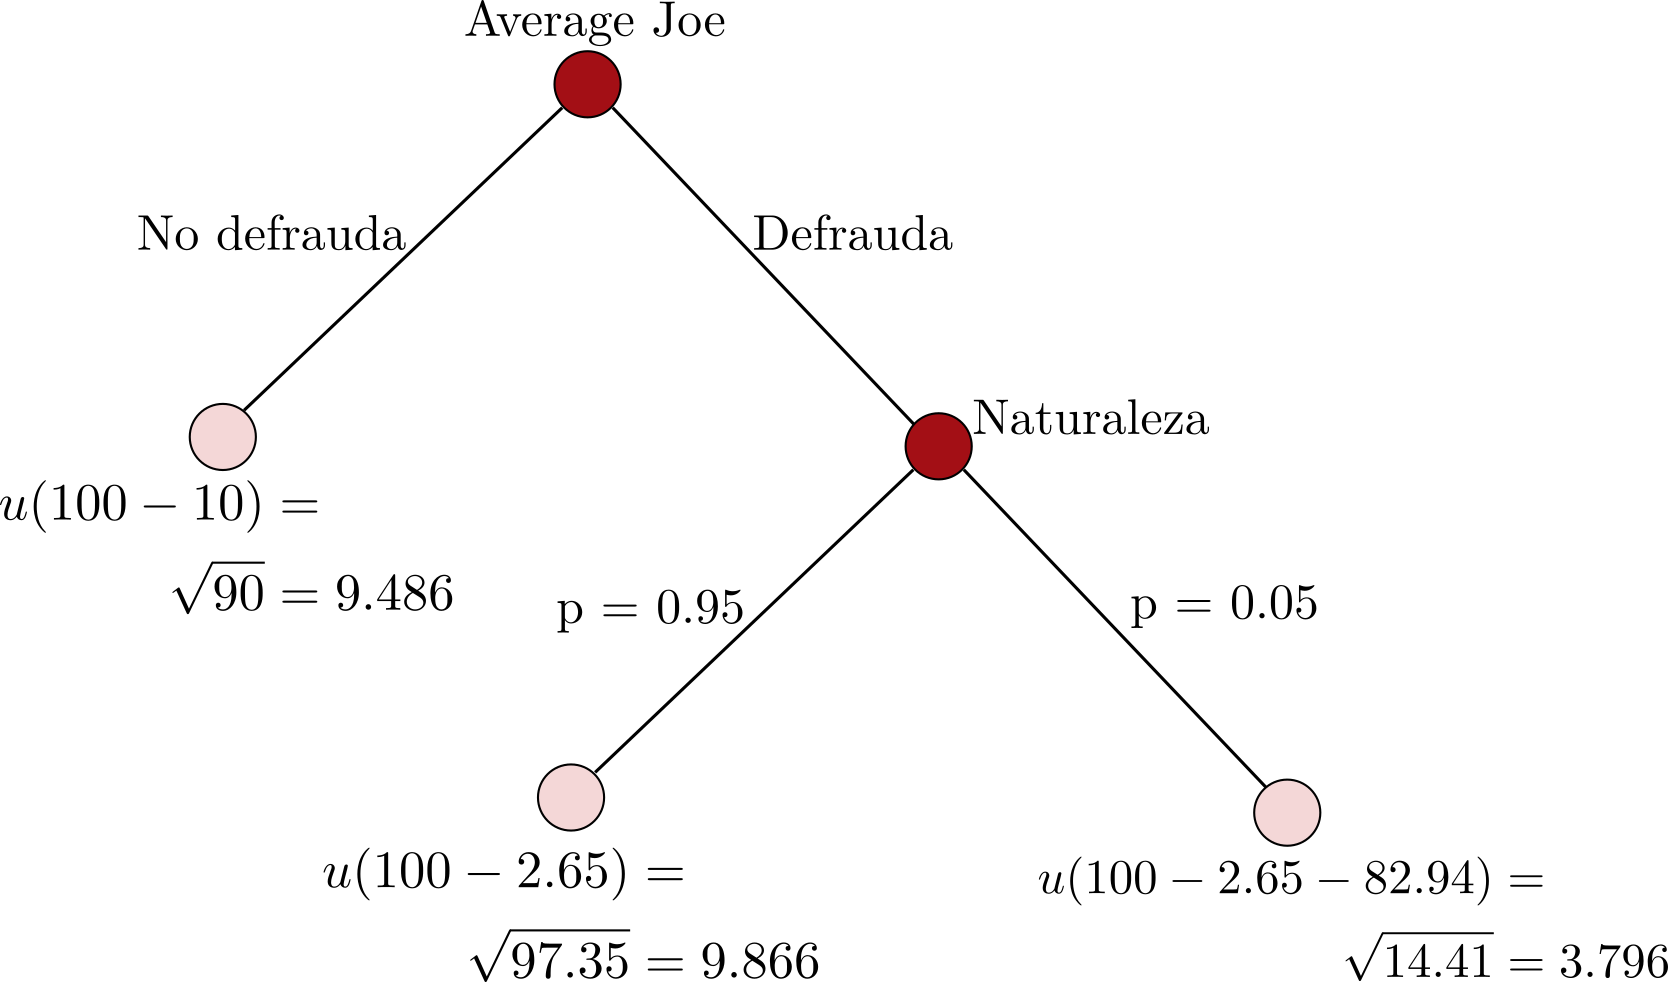
\includegraphics[scale=0.65]{p2tarea1a.png}
          \end{center}
    \item R. Averso. Su función es cóncava.
    \item R.
          \begin{align*}
            U(ND) & = 9.486                                         \\
            UE(D) & = 0.95 \times 9.866 + 0.05 \times 3.796 = 9.562
          \end{align*}

          La utilidad por \textbf{No defraudar} es \textit{menor} que la utilidad por \textbf{Defraudar}.
    \item R.
          \begin{align*}
            U(ND)           & \geq UE(D)                               \\
            9.486           & \geq (1-p) \times 9.866 + p \times 3.796 \\
            9.456-9.866     & \geq 3.79p - 9.866p                      \\
            -0.41           & \geq -6.076p                             \\
            \text{cambiar } & \text{de signo}                          \\
            p               & \geq \frac{0.41}{6.076}                  \\
            p               & \geq 0.067
          \end{align*}

          Si la probabilidad es mayor a 0.067 (o dicho de otra manera, si la proporción de auditados por SAT es mayor al 6.7 \%), sería racional para el individuo cambiar de decisión y no defraudar.

  \end{enumerate}

\end{Exercise}

\begin{Exercise}[name={Respuesta}]

  \begin{enumerate}
    \setlength{\itemsep}{0pt}
    \setlength{\parskip}{0pt}
    \setlength{\parsep}{0pt}

    \item R. El juego en su forma normal es:
          \begin{align*}
            N             & = \{J1, J2\}                    \\
            S             & = q_i \in [0, \infty)           \\
            u_i(q_i, q_j) & = (100  - q_i - q_j)q_i - q_i^2 \\
          \end{align*}
    \item R. Primero definimos el problema como un problema de optimización. \[q_i^* = \argmax_{q_i > 0} u_i(q_i, q_j^*)\]
          Dado que la función de utilidad involucra un término cuadrado en negativo, sabemos que es cóncava, por lo que el C.P.O. es suficiente:
          \[\frac{\partial u_i(q_i, q_j)}{\partial q_i} \Bigr|_{q_j = q_j^*} = 0\]
          \begin{align*}
            \frac{\partial u_i(q_i, q_j)}{\partial q_i} \Bigr|_{q_j = q_j^*} & = 0 \\
            \frac{\partial}{\partial q_i} (100q_i-2q_i^2 -q_iq_j)            & = 0 \\
            100 -4q_i -q_j                                                   & = 0 \\
            % q_i^* &= \frac{100-q_j}{4}\\
          \end{align*}
          Lo que resulta en un sistema de ecuaciones de dos incógnitas:
          \begin{align*}
            100 -4q_1 -q_2  & = 0 \\
            100 -q_1 - 4q_2 & = 0 \\
          \end{align*}
          Resolviendo
          \begin{align*}
            \begin{cases}
              (100 + 4q_1 -q_2 & = 0)\times (-4) \\
              100 + q_1 - 4q_2 & = 0
            \end{cases}
            \iff  \begin{cases}
                    -400 + 16q_1 + 4q_2 & = 0 \\
                    100 -q_1 - 4q_2     & = 0 \\%[-0.2ex]
                    \multispan2{\hrulefill}   \\
                    -300 + 15q_1        & = 0
                  \end{cases} \\
            q_i^* = \frac{300}{15} = 20
          \end{align*}
          El EN es $ (q_1^* = 20, q_2^* = 20) $, con ganancias en equilibrio de $ (800, 800) $.
  \end{enumerate}

\end{Exercise}

\end{document}

